\documentclass{article}
\usepackage{amsmath, amsthm, amssymb, amsfonts, mathtools,enumitem, stmaryrd,physics, cancel, tikz-cd, graphicx, float, booktabs, bbm, mathrsfs}
\usetikzlibrary{arrows}
\usepackage{geometry}
    \geometry{
        a4paper,
        left = 40mm,
        top = 20mm,
        right = 40mm,
        bottom = 30mm
    }
\setlength{\parindent}{0pt}

\theoremstyle{definition}
\newtheorem{problem}{Problem}
\newtheorem{solution}{Solution}
\newtheorem*{example}{Example}
\newtheorem*{exercise}{Exercise}
\newtheorem*{definition}{Definition}
\newtheorem{theorem}{Theorem}
\newtheorem*{theorem*}{Theorem}
\newtheorem{proposition}[theorem]{Proposition}
\newtheorem*{proposition*}{Proposition}
\newtheorem{lemma}[theorem]{Lemma}
\newtheorem*{lemma*}{Lemma}
\newtheorem{corollary}[theorem]{Corollary}
\newtheorem*{corollary*}{Corollary}
\newtheorem*{remark}{Remark}

\title{MAGNTS}
\author{Thanic Nur Samin}


\begin{document}
    \maketitle

    \section*{Saturday, 3/29/2025}
    
    \section*{The algebraic theory of diff eqs by Bjorn Poonen}

    \subsection*{Review of linear DEs}

    Existence and uniqueness theorem for linear ODE:

    \begin{theorem}
        
        Let \(\mathcal{U}\) be a simply connected subset of \(\mathbb{C}\). Let \(\mathcal{O}(\mathcal{U})\) be ring of holomorphic functions \(\mathcal{U} \to \mathbb{C}\)

        \(a\in \mathcal{O}(\mathcal{U}), u\in \mathcal{U}, b\in \mathbb{C}\).

        Then, \(\exists ! f \in \mathcal{O} (\mathcal{U})\) such that \(f^{\prime} = af\) and \(f(u) = b\).

    \end{theorem}

    We also have a version for system (\(n\)-tuple of functions). In that case, we change it to:

    \(A\in M_n(\mathcal{O}(\mathcal{U}))\)

    \(\exists !f\in \mathcal{O}(\mathcal{U})^n\) such that \(f^{\prime} = Af\) and \(f(u) = b\).

    \begin{remark}
        \begin{itemize}
            \item Can replace holomorphic with \(C^{\infty}, \mathbb{C}\) with \(\mathbb{R}\)
            \item Not algebraic: solutions to \(f^{\prime} = z^2 f, f(0)=1\). There exists unique solution: \(f(z)=e^{z^2 / 3}\). But it is not a polynomial.
            \item \(\exists\) nonlinear version but solutions only in a small neighborhood of \(u\). eg \(f^{\prime} =f^2\) with \(f(0)=1\) on \(\mathbb{C}\), solution is \(\frac{1}{1-z}\).
            \item `Simply Connected' is necessarry. Consider \(f^{\prime} = \frac{1}{2z}f\). Seperating variables: \(d(\log f) = \frac{1}{2} d(\log z)\). Has nonzero solution on any simply connected \(\mathcal{U} \subset \mathbb{C}^\times\) [a branch of \(\sqrt{z} \), eg] but no non-zero holomorphic solution on \(\mathbb{C}^\times\).
            \item We can do higher-order differential equations. We convert it into systems of first order differential equation. eg a branch of \(\log z\) on an open subset of \(\mathbb{C}^\times\) is a solution to \((zf^{\prime})^{\prime} = 0\) which we can rewrite as \(f^{\prime\prime} + \frac{1}{2} f^{\prime} = 0\). This is second order, but we can introduce \(g = f^{\prime}\) to get the system \(\begin{dcases}
                f^{\prime} = g\\
                g^{\prime} = -\frac{1}{2}g
            \end{dcases}\). In other words, \(\begin{bmatrix}
                f \\
                g \\
            \end{bmatrix}^{\prime} = \begin{bmatrix}
                0 & 1 \\
                0 & -\frac{1}{2} \\
            \end{bmatrix} \begin{bmatrix}
                f \\
                g \\
            \end{bmatrix}\)
            \item PDEs: \(\exists\) version for functions of \(\geq 2\) variables but it requires an extra `integrability' hypothesis.
            
            Nonlinear Example: \(F(x,y)\) on \(\mathbb{C}^2\) such that \(\frac{\partial F}{\partial x} = y, \frac{\partial F}{\partial y} = -x\). There is going to be no solution to this! The \(y\) derivative of \(\frac{\partial F}{\partial x}\) should be equal to \(x\) derivative of \(\frac{\partial F}{\partial y}\).

            Linear Example: No nonzero \(f(x,y)\) satisfies \(\frac{\partial f}{\partial x} = yf, \frac{\partial f}{\partial y} = - xf\). Proof: If we had a solution, on any open ball where \(f\) is non-vanishingg we can takke a branch of \(\log f\) [call it \(F\)] and this would be a solution to the previous system! Only solution is the \(0\) function.
        \end{itemize} 
    \end{remark}

    \subsection*{Local Systems}

    Let \(X\) be a topological space.

    \(\mathbb{C}^n_{X,\text{pre}}\) is the presheaf such that:

    \begin{definition}
        \begin{enumerate}[label=\roman*)]
            \item For every open \(\mathcal{U} \subset X, \mathbb{C}^n_{X,\text{pre}}(\mathcal{U}) = \mathbb{C}^n\)
            \item The restriction maps are the identity maps  
        \end{enumerate} 
    \end{definition}

    \begin{definition}
        \(\mathbb{C}^n_X\coloneqq\) the sheafification of \(\mathbb{C}^n_{X,\text{pre}}\).
        
        \(\mathbb{C}^n_X(\mathcal{U}) \equiv  \{ \text{\underline{locally} constant functions } \mathcal{U} \to \mathbb{C}^n \}\) 
    \end{definition}

    An automorphism of \(\mathbb{C}_X^n\) as a sheaf of \(\mathbb{C}\)-vector spaces is given by a locally constant function \(X \to \operatorname{GL}_n(\mathbb{C})\) [locally constant change of variable] 

    If \(\phi: Y \to X\) then \(\phi ^{-1} \mathbb{C}_X^n = \mathbb{C}_Y^n\). 

    \begin{definition}
        A local ystem \(\mathcal{L}\) on \(X\) is basically a locally constant sheaf of finite dimensiotnal \(\mathbb{C}\)-vector spaces that,

        \(\exists (U_i)\) open covering on \(X, n_i \in \mathbb{Z}_{\geq 0}, \phi_i : \mathbb{C}_{\mathcal{U}_i}^{n_i} \xrightarrow{\sim} \eval{\mathcal{L}}_{U_i}\)

        We have \(\oplus , \otimes, \operatorname{Hom}\). Get rigid tensor category.
    \end{definition}

    Example: \(\mathcal{L} \simeq \mathbb{C}^n_X\) for some \(n\). Call \(\mathcal{L}\) constant.

    Example \(X = \mathbb{C} ^\times\). For \(\mathcal{U} \subset X,\)

    \[
        \mathcal{L}(\mathcal{U}) \coloneqq \{ \text{solutions to } f^{\prime} = \frac{1}{2z}f \} 
    \]

    Claim: \(\mathcal{L}\) is a \(1\)-dim local system.

    \begin{proof}
        \begin{enumerate}[label=\arabic*)]
            \item If \(\mathcal{U} \subset X\) is simple connected, \(\exists\) branch of \(\sqrt{z}\) on \(\mathcal{U}\).
            \[
                \eval{\mathcal{L}}_{\mathcal{U}} \simeq \mathbb{C}_{\mathcal{U}} \cdot \sqrt{z} 
            \]

            \item \(X\) is covered by such \(\mathcal{U}\).
        \end{enumerate} 
    \end{proof}

    Claim: \(\mathcal{L} \not\simeq \mathbb{C}_X\)

    \begin{proof}
        \(\not\exists\) solution on all of \(X\).
    \end{proof}

    \begin{proposition}
        For any systtem of linear ODES \(f^{\prime} = Af\) as in the uniquness theorem on an open subset of \(\mathbb{C}\), the sheaf of solutions form an \(n\)-dim local systtem.
    \end{proposition}

    \(\mathcal{L}\) local system. Then,

    \underline{fiber of \(\mathcal{L}\) at \(x\in X\)} \(\coloneqq \mathcal{L}_x\) which is \(n\)-dim \(\mathbb{C}\)-vector space.
    
    \begin{figure}[H]
        \centering
        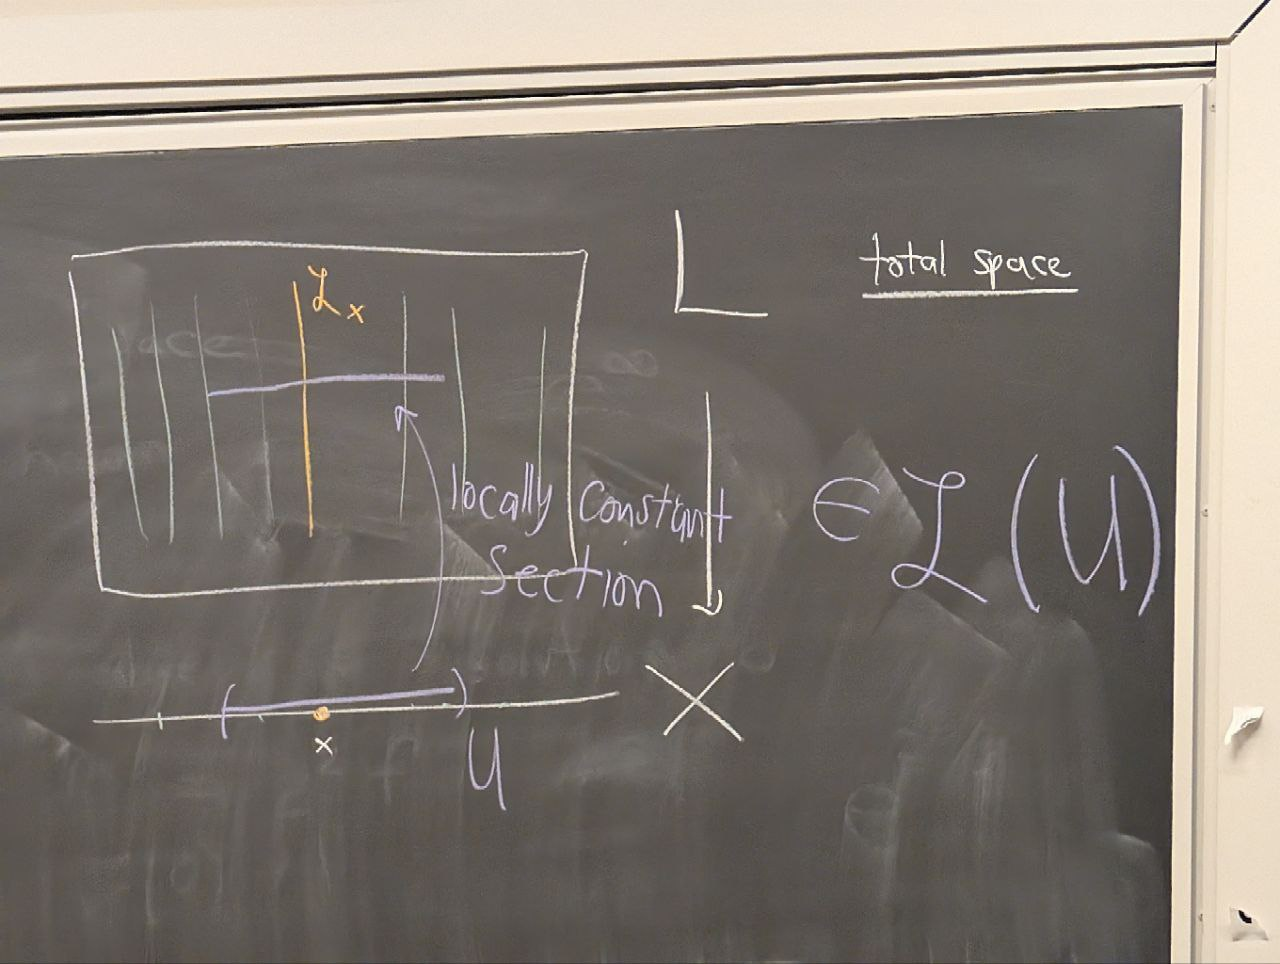
\includegraphics[width=0.8\textwidth]{img/fiberL}
    \end{figure}

    Example (Relative Betti Cohomology)

    \(X\) compact \(C^{\infty}\)-manifold.

    \(\Gamma (X,-)\) 

    \(H^q(X,-)\)

    \(H^q(X,\mathbb{C})\) fin dim \(\mathbb{C}\)-vector space.

    \(X \to B\) prooper submersion of \(C^{\infty}\) manifolds.

    \(\pi_{\ast}\) 

    \(R^q \pi_{\ast}\) 

    \((R^q \pi_{\ast}) \mathbb{C}_X\) sheaf of \(\mathbb{C}\)-vector spaces  on \(B\).

    This is a local system on \(B\).

    \((R^q \pi_*\mathbb{C}_X)_b = H^q(X,\mathbb{C})\)

    \begin{figure}[H]
        \centering
        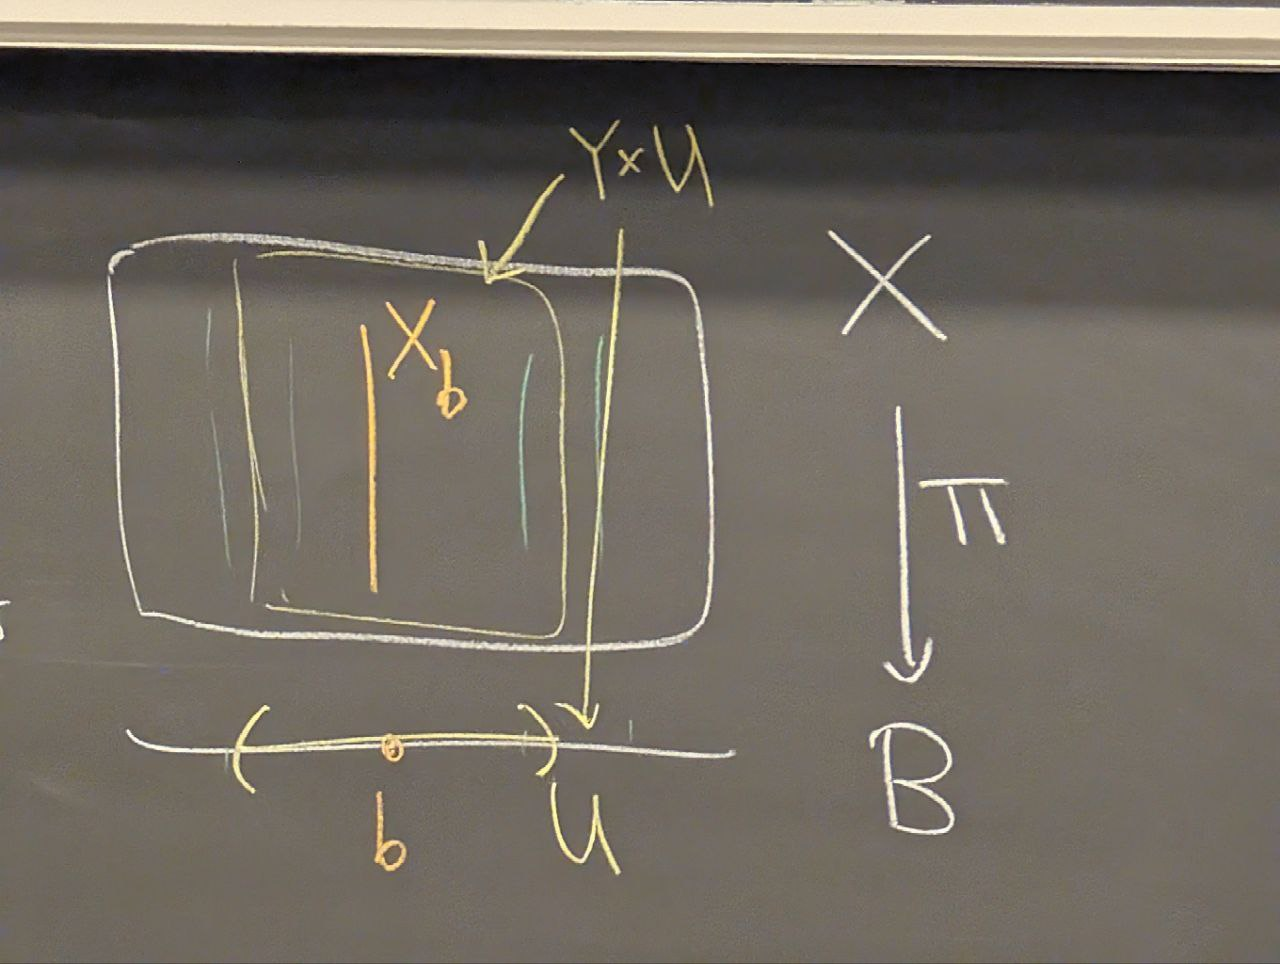
\includegraphics[width=0.8\textwidth]{img/betticohom}
    \end{figure}

    Question: What does a local system on \([0,1]\) look like?

    \begin{proposition}
        Let \(\mathcal{L}\) be a local system on \([0,1]\). Then,

        \begin{enumerate}[label=\alph*)]
            \item \(\mathcal{L}\) is constant [proof: open cover to finite subcover, these overlap, we keep changing variables by \(\operatorname{GL}_n\) on overlaps and get a constant function on the whole thing.]
            
            \item \(\mathcal{L}_0 \simeq \mathcal{L}_1\) [we can naturally identify fibers on \(0\) to fibers at \(1\)].
        \end{enumerate} 
    \end{proposition}

    \subsection*{Local systems and reps of \(\pi_1\)}

    \(\gamma: [0,1] \to X\) path from \(x\) to \(y\).

    If we have local system \(\mathcal{L}\) on \(X\) we can pull it back to the interval. Then, \(\gamma ^{-1} \mathcal{L}\) is constant. Fibers of \(0,1\) [meaning fibers of \(x,y\)] gives us isomorphism \(\mathcal{L}_x \simeq \mathcal{L}_y\).

    If we deform the path into a homotopic one then we get the same isomorphism.

    This gives us:

    \[
        \frac{\{ \text{paths from \(x\) to \(y\)}  \}}{\text{homotopy}} \times \mathcal{L}_x \to \mathcal{L}_y
    \]

    Take \(y=x\). Then our paths are loops.

    We get \(\pi_1(X,x)\) action on \(\mathcal{L}_x\) in this case. This is a representation of this group. This is called the monodromy representation: \(\mathcal{L}_x\) with action of \(\pi_1(X,x)\)

    We also have monodromy group: \(\operatorname{im} \left( \pi_1(X,x) \to \operatorname{GL}(\mathcal{L}_x)\right) \) 

    If we go back to the square root example, take \(X=\mathbb{C}^\times, x = 1\)

    \(\pi_1(\mathbb{C}^\times, 1) = \mathbb{Z}\) 

    Then \(\mathcal{L} = \text{solutions to } f^{\prime} = \frac{1}{2z}f\).

    The we have \(\pi_1(\mathbb{C}^\times,1) \to \operatorname{GL}(\mathcal{L}_x) = \mathbb{C}^{\times}\)

    \([\gamma] \mapsto -1\)

    So, the monodromy group would be \(\pm 1\).

    \begin{theorem}
        Let \(X\) connected, locally simply connected topological space. Then, the functor

        \[
            \{ \text{local systems on } X \} \to \{ \text{fin dim reps of } \pi_1(X,x) \}  
        \]

        \[
            \mathcal{L} \mapsto \mathcal{L}_x \text{ with its \(\pi_1(X,x)\)-action} 
        \]

        is an equivalence of tensor categories.
    \end{theorem}

    Idea of proof: Pull back the local system of the universal cover and a bunch of other stuff.

    \section*{Random Walks in NT by Koukoulopoulus}

    \begin{itemize}
        \item \(\omega(n) = \#\{ p \mid n \} = \sum_{p} \mathbbm{1}_{p\mid n} \implies 2^{\omega(n)} \approx \tau (n) = \#\{ d\mid n \} \)
        \item \(\log (\zeta (s)) \approx \sum_{p} \frac{1}{p^s}\). \(e^{\log \zeta (s)} = \zeta(s)\)    
    \end{itemize}
    
    Think of them as RVs.

    \begin{itemize}
        \item \(\{ n \leq x \}\) probability space equipped with the uniform counting measure.
        \item Fix \(\sigma\), vary \(t\in [T,2T]\) equippe wiith lebesgue measure.
        
        \(B_p(n) = \mathbbm{1}_{p\mid n}\) Bernoulli RV.

        \(\mathbb{P}(B_p = 1) = \frac{\#\{ n \leq x, p\mid n \}}{\#\{ n \leq x \} } = \frac{\lfloor x / p \rfloor}{\lfloor x \rfloor} = \frac{1}{p} + O(1 / x) \sim \frac{1}{p}\) 
    \end{itemize} 

    \(p^{-it} \in S^1 \rightsquigarrow \approx\) unfirom dist on \(S^1\)  
    
    \(e^{-it \log p}\) is \(\frac{1}{\log p}\)-periodic.

    \(= e^{-i \{ t\log p \} }\) 

    \(\operatorname{meas}(t\in [T,2T]) = t \log p \in [a,b] (\mod 2\pi) \approx \frac{b-a}{2\pi} \cdot T\) 

    We want to take \(k\) different primes \(p_1 < \cdots < p_k\) and want to understand what is the joint distribution of \(B_{p_1}, \cdots , B_{p_k}\).

    \(\mathbb{P}(B_{p_1} = \cdots = B_{p_{k}} = 1) \sim \frac{1}{p_1 \cdots p_k} \sim \prod_{j=1}^{k} P(B_{p_j}) = 1\).
    
    Thus, \(B_{p_1}, \cdots , B_{p_k}\) are approximately independent of each other.

    \(\mathbb{E}[B_p] \sim \frac{1}{p}\) 

    \(\operatorname{Var}[B_p] = \frac{1}{p} - \frac{1}{p^2} \)
    
    Thus, \(E[\sum_{p \leq x} B_p] \sim \sum_{p \leq x} \frac{1}{p} \sim \log_2 x\)
    
    \(\operatorname{Var}[\sum_{p \leq x} B_p] = \sum_{p \leq x} \frac{1}{p} - \frac{1}{p^2} \sim \log_2 x\) 

    \begin{theorem}
        [Erd\"os-Kac Theorem]

        \[
            \frac{\omega(n) - \log_2 x}{\sqrt{\log_2 x}} \overset{d}{\implies} \mathcal{N}(0,1)
        \]
    \end{theorem}

    \begin{definition}
        \(X_n \overset{d}{\implies} X \iff \forall \phi \in C_c^{\infty} (R), \mathbb{E}[\phi(X_n)] \to \mathbb{E}[\phi(X)] \iff \mathbb{P}(X_n \leq a) \to \mathbb{P} (X \leq a) \forall u\) that is a point of the continuity of the latter.
    \end{definition}

    \[
        \forall u\in \mathbb{R} , \# \left\{ n \leq x : \frac{\omega(n) - \log_2 x}{\sqrt{\log_2 x} } \leq u \right\} \sim x \cdot \frac{1}{\sqrt{2\pi}} \int_{-\infty}^{u} e^{-t^2 / 2} \,\mathrm{d}t 
    \]

    Let \(p_1 < \cdots < p_k\). let \(m_1, \cdots , m_k \in \mathbb{Z}\) Then,

    \[
        \frac{1}{T} \int_{T}^{2T} (p_1^{it})^{m_1} \cdots (p_k^{it})^{m_k} \,\mathrm{d}t 
    \]

    \[
        = \frac{1}{T} \int_{T}^{2T} e^{it (\underbrace{m_1 \log p_1 + \cdots + m_k \log p_k}_{\theta})} \,\mathrm{d}t 
    \]

    Use the fact: \(\int_{T}^{2T} e^{i \theta t} \,\mathrm{d}t = \frac{e^{i \theta 2T} - e^{i \theta T}}{i \theta} = O(\frac{1}{\vert \theta \vert})\) 

    \[
        = \begin{dcases}
            1, &\text{ if } m_1 \log  p_1 + \cdots + m_k \log p_k = 0 ;\\
            \frac{1}{T} \frac{1}{\vert m_1 \log p_1 + \cdots + m_k \log p_k \vert}, &\text{ otherwise} .
        \end{dcases}
    \]

    If \(\exists m_i \neq 0\) then \(m_1 \log p_1 + \cdots + m_k \log p_k = \log \frac{a}{b}\). \(a,b\in \mathbb{N}\)
    
    \(a,b \leq p_1^{\vert m_1 \vert} \cdots p_k^{\vert m_k \vert} \leq y^{kM}\) if \(\vert m_i \vert \leq M, p_i \leq y\)
    
    \(\vert \log \frac{a}{b} \vert \gg \frac{1}{y^{kM}}\) 

    \(y = T^{\frac{1}{\log _2 T}}\), \(k,M \leq (\log_2 T)^{1 / 3}\)  

    \(\mathbb{E} \left[ \frac{p^{it}}{p^\sigma} \right] = 0, \operatorname{Var} (\frac{p^{it}}{p^\sigma}) = \frac{1}{p^{2\sigma}} = \begin{dcases}
        \sum_{p} \frac{1}{p^{2\sigma}} = \infty, &\text{ if } \sigma = \frac{1}{2} ;\\
        \sum_{p} \frac{1}{p^{2\sigma}} < \infty, &\text{ if } \sigma > \frac{1}{2} ;
    \end{dcases}\) 

    Small primes are too important, so we don't have CLT.

    \begin{theorem}
        [Selben's CLT]

        \[
            \frac{\log \zeta (\frac{1}{2} + it)}{\sqrt{\log_2 T}} \overset{d}{\implies} N_\mathbb{C}(0,1) = N_{\mathbb{R}}(0,\frac{1}{2}) + i N{\mathbb{R}}(0,\frac{1}{2})
        \]

    \end{theorem}

    \(\forall u\in \mathbb{R}\)

    \(\operatorname{meas} \left( t\in [T,2T] : \log \vert \frac{1}{2} + it \vert \leq u \sqrt{\frac{1}{2} \log_2 T}  \right) \sim \frac{T}{\sqrt{2T}} \int_{-\infty}^{u} e^{-v^2 / 2} \,\mathrm{d}v\) 

    \subsection*{Detour to Probability Theory}

    Suppose \(X_1, X_2, \cdots\) are ind real RVs

    \(\mu_1 = \mathbb{E}[X_i], \sigma_i^2 = \operatorname{Var}[X_i]\) 

    \(s_n^2 = \sigma_1^2 + \cdots + \sigma_n^2 = \operatorname{Var}(X_1, \cdots , X_n)\) 

    Lindeberg Condition: 

    \[
        \frac{1}{s_n^2} \sum_{j=1}^n \mathbb{E} \left[ (X_j - \mu_j)^2 \cdot \mathbbm{1}_{\vert X_j - \mu_j \vert > \epsilon s_n}\right] \to 0 
    \]

    Then \(\frac{X_1 + \cdots + X_n - \mu_1 - \cdots - \mu_n}{s_n} \overset{d}{\implies} \mathcal{N}(0,1)\) 

    We use method of moments, see Billingsley.

    Now we prove Erd\"os=Kac

    \begin{proof}
        Consider perfect random walk.

        \(\forall p, B_p^{\text{Model}}\) is Bernoulli, \(\mathbb{P}(B_p^{\text{Model}} = 1) = \frac{1}{p}\)  i.i.d.\  of each other.

        CLT \(\implies \frac{\sum_{p \leq y} B_p^{\text{Model}} - \log \log p}{\sqrt{\log_2 y} } \overset{d}{\implies} \mathcal{N}(0,1)\) as \(y \to \infty\)
        
        \(\omega(n) = \# \{ p\mid n, p \leq x \} = \# \{ p \mid n, p \leq x \} + O \left( \frac{\log x}{\log y} \right)\). 

        \[
            \sum_{n \leq x} \omega(n)^2 = \sum_{n \leq x} \sum_{p_1 p_2 \mid n} = \sum_{p_1 p_2 \leq x} \# \{ n \leq x, p_1 p_2 \mid n \} 
        \]

        \(p_2, p_2\) could be too large \(p_1, p_2 \approx x^{\frac{2}{3}}\).

        Idea: choose \(y\) cleverly in \(\omega(n) = \# \{ p\mid n, p \leq x \} = \# \{ p \mid n, p \leq x \} + O \left( \frac{\log x}{\log y} \right)\).

        We choose \(y = x^{1 / \log_3 x}\) 

        \[
            \sum_{n \leq x} \omega(n,y)^k = \sum_{n \leq x} \sum_{p_1, \cdots, p_k \leq y, p_1, \cdots , p_k \mid n} 1
        \]

        \[
            = \sum_{p_1, \cdots , p_k \leq y} \left( \frac{x}{[p_1, \cdots , p_k]} + O(1) \right)  
        \]

        total error \(y^k = o(x)\) 

        \[\equiv x \mathbb{E} [B_p^{\text{Model}}]\] 

    \end{proof}

    \section*{The algebraic theory of diff eqs by Bjorn Poonen 2}

    \subsection*{Vector Bundles}

    \(X\) complex manifold

    \(m = \dim X\) 

    \(\mathcal{O} = \mathcal{O}_X\), sheaf of holomorphic functions.

    \begin{definition}
        Vector bundle on \(X \coloneqq\) locally free \(\mathcal{O}\)-modules that is locally of finite rank.
    \end{definition}


    \begin{table}[H]
        \centering
        \begin{tabular}{c|c}
            \toprule
                Vector Bundle & Rank \\
            \midrule
                \(\mathcal{O}\) & \(1\)  \\
                Tangent Bundle \(\mathcal{T}\)  & m \\
                Sheaf of \(1\)-forms \(\Omega^1 \coloneqq \operatorname{Hom}(\mathcal{T} , O)\) & m \\
            \bottomrule
        \end{tabular}
        \caption{Rank of Vector Bundles}
    \end{table}

    For each \(x\in X\) we get:

    \begin{itemize}
        \item The \underline{stack{ \(V_{(\ast)}\) }} which is a finite free \(\mathcal{O}_{(\ast)}\) module
        \item Thee fiber \(V_{\ast} \coloneqq V \otimes_{\mathcal{O}} k_\times = V_{(\ast)} / m_{\ast} V_{(\ast)}\) which form a fin. dim \(\mathbb{C}\)-vector space.   
    \end{itemize} 

    Example: \(\mathcal{L}\) local system, \(\mathcal{V} \coloneqq \mathcal{O} \otimes_{\mathbb{C}} \mathcal{L}, \mathcal{L}_{\ast} = V_{\ast} \)

    \(\mathcal{L} =\) sheaf of  locally constant functions. 

    \(V =\) sheaf of all holomorphic function.

    \subsection*{Derivations}

    \(A\) is \(\mathbb{C}\)-algebra.

    \begin{definition}
        [Derivation of \(A\)]:\(A\) \(\mathbb{C}\)-algebra.

        Derivation of \(A\): a \(\mathbb{C}\)-lindar map \(D: A \to A\) such that \(D(fg) = D(f)g + f D(g)\) for all f\(,g\in A\).


        eg \(\frac{\partial}{\partial x}, y^2 \frac{\partial}{\partial x}\) 

    \end{definition}

    As sheafs of \(\mathbb{C}\)-algebrras

    Derivation \(D\) of \(A =\) collection \((D_u)_{u \subset X}\) such that \(D_u\) is a derivation of \(A(\mathcal{U})\) compatible with the restriction.

    \(\operatorname{Der} (\mathcal{A}) = \{ \text{all derivations of } \mathcal{A} \}   \)
    
    \(\mathscr{D}er(A) = \) the sheaf \(\mathcal{U}\to \operatorname{Der}(\eval{A}_u)\)  

    For each vector field function \(t\in \mathcal{T} , f\in \mathcal{O} , x\in X\) 

    Let \((D_t f)(x) \coloneqq\) directional derivative of \(f\) in the diretion of \(t(x)\) 

    \(D_t f \in \mathcal{O}\) 

    Get \(T \xrightarrow{\sim} \mathscr{D}er, t \mapsto D_t\) 

    The pairing \(\mathcal{T} \times \mathcal{O} \to \mathcal{O}\) given by \(t, f \mapsto D_t f\)
    
    \(\mathcal{O}\)-linear in \(t\), \(\mathbb{C}\)-linear in \(f\). Get:

    \(\mathcal{O} \xrightarrow{d} \operatorname{Hom}(\mathcal{T} , \mathcal{O}) \eqqcolon \Omega^1\)
    
    \(1 \mapsto df\).

    \(V \simeq \mathcal{O}_x \xrightarrow{e^{z^{\prime}}} \mathcal{O}_x\) 

    \(v \mapsto 1 \mapsfrom e^z\) 

    To equip \(V\) with a rule for taking directional derivatives of of sections of \(V\) we should specify a pairing
    
    \(T \times V \to V, t,v \mapsto \nabla_t v, \operatorname{Home}(T,V)\).
    
    \(\nabla: V \to \operatorname{Hom}(T,V) = \Omega^1 \otimes V\)
    
    Given \((\gamma , \delta)\) , each \(D \in \mathscr{D}er(X) = T(X) = \operatorname{Hom}(\Omega^1, 0)\) induces:

    \[
        \nabla_D : \mathcal{V} \xrightarrow{\nabla} \Omega^1 \otimes V \xrightarrow{D \otimes 1} \mathcal{O} \cdot V = V
    \]

    eg \(d\) is a connection on \(\mathcal{O}\)
    
    eg \(\omega \in \Omega^1(X)\)
    
    \(d+\omega : \mathcal{O} \to \Omega^1, f \mapsto df + f \omega\)
    
    \begin{proposition}
        Every connection on \(\mathcal{O}\) is \(d+\omega\) for some \(\omega \in \Omega ^1(X)\) 
    \end{proposition}

    \begin{proof}
        Let \(\nabla\) be a connection on \(\mathcal{O}\). Then,

        \[
            \nabla(fg) = df g + f \nabla g
        \]

        \[
            d(fg) = df g + f dg
        \]
    \end{proof}

    \((\nabla - d)(fg) = f(\nabla - d) g\) 

    Thus, \(\nabla - d\) is \(\mathcal{O}\)-linear hence \(\mathcal{O} \to \Omega^1, f \mapsto f \omega\) for some \(\omega \in \Omega ^1(X)\) 

    We also have: every connection on \(\mathcal{O}^n\) is \(d+ \omega\) for some \(\omega \in \Omega^1(X)\).

    Fix \((V,\nabla)\).

    \(v\in V\) is called horizontal if \(\Delta v = 0\).

    \(V^\nabla \coloneqq \ker\nabla \subset V\).

    subsheaf of horizontal schemes

    eg \(\mathcal{U} \subset \mathbb{C}, V = \mathcal{O}^n, A \in M_n(\mathcal{O}(\mathcal{U})), \nabla = d - A dz\)
    
    Then horizontal schems of \(V =\) solutions \(f\in \mathcal{O}^n\) to the system \(f^{\prime} = Af\) 

    eg \(X = \mathbb{C} , V = \mathcal{O} , \nabla = d - z^2 \, \mathrm{d} z\)
    
    \(\nabla f = df - fz^2 \, \mathrm{d}z\) 

    So \(\nabla f = 0 \iff f^{\prime} = z^2 f\)
    
    \(\gamma^\nabla = \mathbb{C}_x \cdot e^{z^3 / 3}\) 

    \begin{proposition}
        \(\dim X = 1, (V,\nabla)\) on \(X\). Then, \(V^\nabla\) is a \(n\)-dim local system on \(X\). 
    \end{proposition}

    \subsection*{Curvature}

    \(\nabla\) on \(V\) induces a seq of \(\mathbb{C}\)-lienar maps.

    \[
        V \xrightarrow{\nabla} \Omega^1 \otimes_ V \xrightarrow{\nabla_1} \Omega^2 \otimes V \to \cdots 
    \]

    Where \(\nabla_i(\omega \otimes v) = d \omega v + (-1)^i \omega \otimes v\) 

    The curvture of \(\nabla\) is:

    \(K \coloneqq \nabla_1 . \nabla: V \to \Omega^2 \otimes V\)
    
    It turns out that \(K\) is \(\mathcal{O}\)-linear so \(K\) is a global section of

    \[
        \operatorname{Hom}(V, \Omega^2 \otimes V) = \Omega^2 \otimes \operatorname{End}(V) 
    \]

    \(\nabla\) is an integrable connection, a flat connection if and only if \(K = 0\)
    
    eg If \(\dim X = 1\) then \(\Omega ^2 = 0\) so \(K = 0\) automatically.

    eg If \((V,\nabla) = (0,d)\) then

    \[
        \mathcal{O} \xrightarrow{d} \Omega^1 \xrightarrow{d} \Omega^2 0>\cdots 
    \]

    is the usual de Rham complex.

    eg If \((V,\nabla) = (\mathcal{O}, d+\omega)\)
    
    \(K(1) = \nabla_1(\nabla 1) = \nabla_1 \omega = d \omega\) 

    So \(K = d \omega\) 

    \(\nabla\) is integrable \(\iff \omega\) is a closed \(1\)-form.

    eg Let \(X = \mathbb{C}^2\) with coords \(x,y, V = 0, \omega = -y \, \mathrm{d}x  + x dy \in \Omega^1(X)\) 

    Let \(\nabla = d + \omega\) then \(K = d \omega \equiv  2 \mathrm{d} x \wedge \mathrm{d} y \neq 0\). \(\nabla\) is not integrable.

    \(V^\nabla\) is sheaf of solutions to \(df + \omega f = 0 \) so no nonzero solutions.
    
    \(V^\nabla = 0\) 

    \section*{Random Walks in NT by Koukoulopoulus 3}

    Recall:

    \(\omega(n) = \sum_{p \leq x} \mathbbm{1}_{p\mid n} \approx \sum_{p \leq y} \mathbbm{1}_{p\mid n}, y = x^{1 / \log_3 x}\) 

    \(\log \vert \zeta (\frac{1}{2} + it) \vert \approx \log \vert \zeta(\frac{1}{2} + \frac{1}{\log y} + it) \vert \approx \sum_{p \leq y} \frac{1}{p^{\frac{1}{2} + it}} \, y = T^{1 / \l\log _3 T} , t\in [T,2T]\) 

    \(X_1, X_2, \cdots \) i.i.d.\  mean \(0\), var \(1\).

    \(\frac{X_1 + \cdots + X_n}{\sqrt{N}} \implies N(0,1)\)
    
    \(f_N(\alpha) = \frac{1}{\sqrt{N}} \sum_{n \leq \alpha N} X_n\), \(\operatorname{Var} (f_N) = \frac{\alpha N}{N} = \alpha \implies N(0,\alpha)\)
    
    \(f_N(\beta) - f_N(\alpha) = \frac{1}{\sqrt{N}} \sum_{\alpha N < n \leq \beta N} X_n \implies N(0,\beta - \alpha)\).
    
    \(f_N\): brownian motion.

    \begin{theorem}
        [Billingsley] If \(n\) simple uniform random from \([1,x]\cap \mathbb{Z}\), then the stochastic process \(g: [0,1]\to \mathbb{R}\),
        
        \[
            g(\alpha) = \frac{\# \{ p\mid n, \log_2 p \leq  \alpha \log_2 x \} - \alpha \log_2 x }{\sqrt{\log_2 x} } 
        \]

        So brouwnian motion on \([0,1]\).
    \end{theorem}

    What is the distribution of \(g\) if we condition on \(n\) having \(r= \rho \log_2 x, \rho =\) constant.
    
    Convergene to brownian bridge \(=\) brownian motion given end propbability \(= 0\).

    \subsection*{Maximum of \(\zeta\)}

    \(\max_{t\in [T,2T]} \log  \left\vert \zeta \zeta (\frac{1}{2} + it) \right\vert \sim \sqrt{\frac{1}{2} \log T \log_2 T} = \sqrt{\log T} \cdot \sqrt{\frac{1}{2} \log_2 T}   \) 

    Conjeture (Farner-Gortek Hughes)

    \(\frac{1}{T} \int_{T}^{2T} \vert \zeta(\frac{1}{2} + it) \vert^{2k}  \,\mathrm{d}t \sim \frac{1}{2}C_k(\log T)^{k^2} \)

    dominated by \(\log \vert \zeta \vert \) 

    Conj of Fyodorov-Hiary--Keating about the distribution of the local maximum.

    \(M(t) \coloneqq \max_{h\in [0,1]} \log \vert \zeta(\frac{1}{2} + i(t+h) ) \vert \) 

    Dostrobution of \(M(t)\) when \(t\) in uniform \([T,2T]\)

    Conjecture: \(M(t) = \log_2 T - \frac{3}{4} \log_3 T + O(1)\) a.s.
    
    \(\log \vert \frac{1}{2} + i(t+h) \vert \approx k \sum_{p \leq T} \frac{1}{p^{1 / 2} + it + ih} \to S(h) = \sum_{p \leq T} \text{Re} \frac{X_p}{p^{1 / 2 + ih}} \) where \(X_p = \text{Unit}(S^1)\) mutually independent. \(p^{it} \approx \operatorname{Uniform}(S)\).
    
    \(\mathbb{E} [S(h_1)S(h_2)] = \sum_{p_1, p_2 \leq T} \mathbb{E} \left[ \text{Re} \frac{X_{p_1}}{p^{\frac{1}{2} + ih_1}} \text{Re} \frac{X_{p_2}}{p^{1 / 2} + ih_2} \right]  \) 

    \(= \frac{1}{4} \sum_{p \leq T} \left( \frac{1}{p^{1+i(h_1 - h_2)}} + \frac{1}{p^{1+i(h_2 - h_1)}} \right) = \begin{dcases}
        \frac{1}{2} \log_2 T, &\text{ if } \vert h_1 - h_2 \vert \leq \frac{1}{\log T} ;\\
        0, &\text{ if } \vert h_1 - h_2 \vert \gg 1  ;\end{dcases}\) 


    Easier Problem:

    \(\max (Z_1, \cdots ,Z_N)\)
    
    \(Z_i \sim N(0, \frac{1}{2} \log_2 T, N = \l \log T)\).
    
    \(\mathbb{P} \max_{1 \leq i \leq N} Z_i \leq \mu\)
    
    \(= \mathbb{P} (Z_i \leq \mu)^N\) 

    \(= \left( 1 - \mathbb{P} (Z_1 > \mu) \right)^N \) 

\end{document}